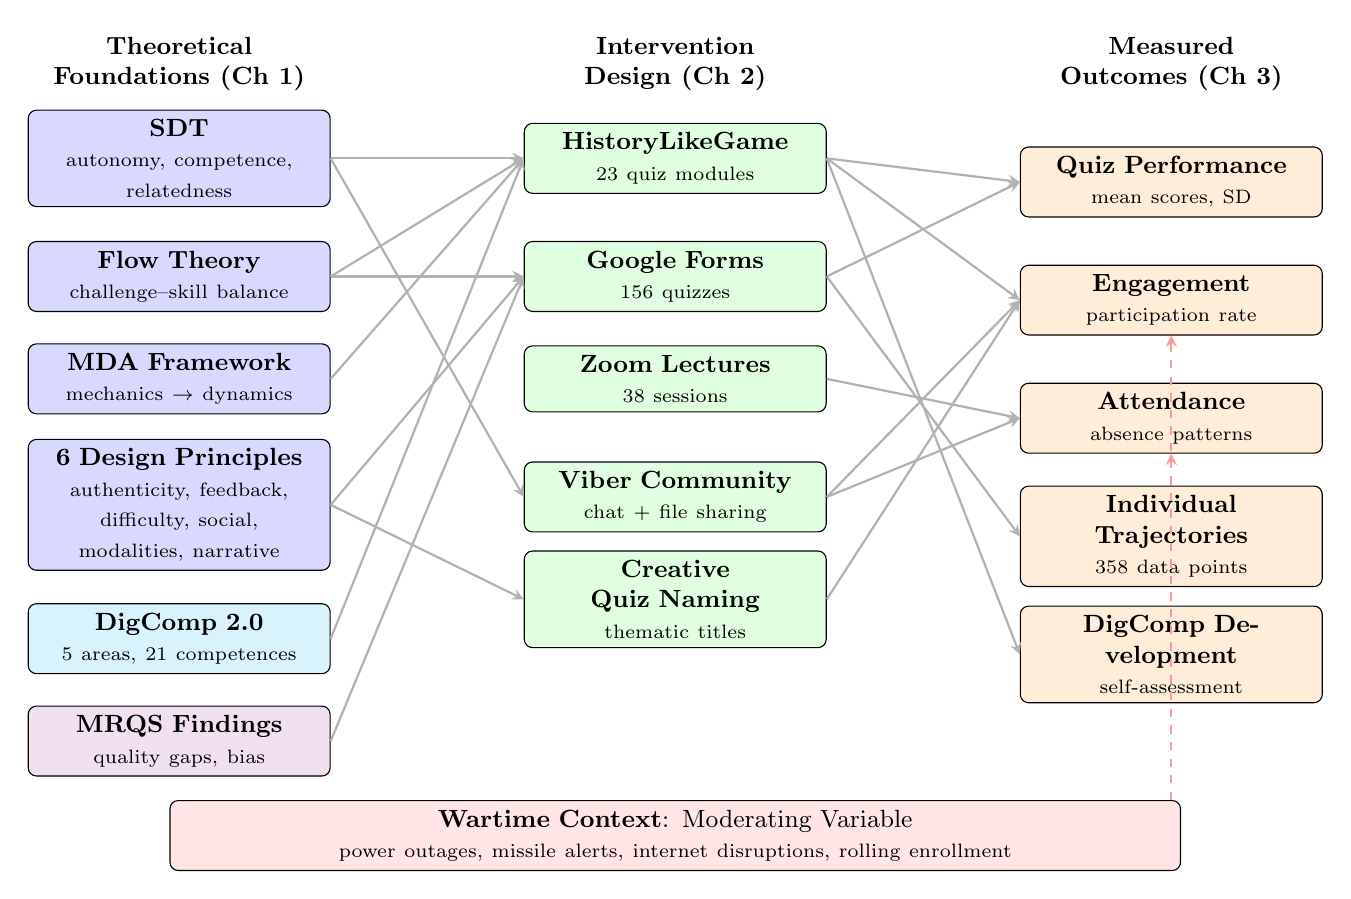
\begin{tikzpicture}[
  node distance=0.4cm,
  theorybox/.style={rectangle, draw, rounded corners=3pt, fill=blue!15,
    text width=3.6cm, minimum height=0.7cm, align=center, font=\small},
  intbox/.style={rectangle, draw, rounded corners=3pt, fill=green!12,
    text width=3.6cm, minimum height=0.7cm, align=center, font=\small},
  outbox/.style={rectangle, draw, rounded corners=3pt, fill=orange!15,
    text width=3.6cm, minimum height=0.7cm, align=center, font=\small},
  colhead/.style={font=\bfseries\small, align=center},
  arr/.style={->, >=stealth, thick, gray!60},
  warbar/.style={rectangle, draw, rounded corners=3pt, fill=red!10,
    minimum height=0.7cm, align=center, font=\small}
]

% Column headers
\node[colhead] (h1) at (0, 0) {Theoretical\\Foundations (Ch~1)};
\node[colhead] (h2) at (6.3, 0) {Intervention\\Design (Ch~2)};
\node[colhead] (h3) at (12.6, 0) {Measured\\Outcomes (Ch~3)};

% Column 1: Theory
\node[theorybox] (sdt) at (0, -1.2) {\textbf{SDT}\\{\scriptsize autonomy, competence,}\\{\scriptsize relatedness}};
\node[theorybox] (flow) at (0, -2.7) {\textbf{Flow Theory}\\{\scriptsize challenge--skill balance}};
\node[theorybox] (mda) at (0, -4.0) {\textbf{MDA Framework}\\{\scriptsize mechanics $\to$ dynamics}};
\node[theorybox] (principles) at (0, -5.6) {\textbf{6 Design Principles}\\{\scriptsize authenticity, feedback,}\\{\scriptsize difficulty, social,}\\{\scriptsize modalities, narrative}};
\node[theorybox, fill=cyan!15] (digcomp) at (0, -7.3) {\textbf{DigComp 2.0}\\{\scriptsize 5 areas, 21 competences}};
\node[theorybox, fill=violet!12] (mrqs) at (0, -8.6) {\textbf{MRQS Findings}\\{\scriptsize quality gaps, bias}};

% Column 2: Intervention
\node[intbox] (hlg) at (6.3, -1.2) {\textbf{HistoryLikeGame}\\{\scriptsize 23 quiz modules}};
\node[intbox] (gforms) at (6.3, -2.7) {\textbf{Google Forms}\\{\scriptsize 156 quizzes}};
\node[intbox] (zoom) at (6.3, -4.0) {\textbf{Zoom Lectures}\\{\scriptsize 38 sessions}};
\node[intbox] (viber) at (6.3, -5.5) {\textbf{Viber Community}\\{\scriptsize chat + file sharing}};
\node[intbox] (naming) at (6.3, -6.8) {\textbf{Creative Quiz Naming}\\{\scriptsize thematic titles}};

% Column 3: Outcomes
\node[outbox] (perf) at (12.6, -1.5) {\textbf{Quiz Performance}\\{\scriptsize mean scores, SD}};
\node[outbox] (engage) at (12.6, -3.0) {\textbf{Engagement}\\{\scriptsize participation rate}};
\node[outbox] (attend) at (12.6, -4.5) {\textbf{Attendance}\\{\scriptsize absence patterns}};
\node[outbox] (traj) at (12.6, -6.0) {\textbf{Individual Trajectories}\\{\scriptsize 358 data points}};
\node[outbox] (dcomp) at (12.6, -7.5) {\textbf{DigComp Development}\\{\scriptsize self-assessment}};

% Arrows: Theory → Intervention
\draw[arr] (sdt.east) -- (hlg.west);
\draw[arr] (sdt.east) -- (viber.west);
\draw[arr] (flow.east) -- (hlg.west);
\draw[arr] (flow.east) -- (gforms.west);
\draw[arr] (mda.east) -- (hlg.west);
\draw[arr] (principles.east) -- (gforms.west);
\draw[arr] (principles.east) -- (naming.west);
\draw[arr] (digcomp.east) -- (hlg.west);
\draw[arr] (mrqs.east) -- (gforms.west);

% Arrows: Intervention → Outcomes
\draw[arr] (hlg.east) -- (perf.west);
\draw[arr] (hlg.east) -- (engage.west);
\draw[arr] (gforms.east) -- (perf.west);
\draw[arr] (gforms.east) -- (traj.west);
\draw[arr] (zoom.east) -- (attend.west);
\draw[arr] (viber.east) -- (attend.west);
\draw[arr] (viber.east) -- (engage.west);
\draw[arr] (naming.east) -- (engage.west);
\draw[arr] (hlg.east) -- (dcomp.west);

% Bottom bar: Wartime context (moderating variable)
\node[warbar, text width=12.6cm] (war) at (6.3, -9.8) {\textbf{Wartime Context}: Moderating Variable\\{\scriptsize power outages, missile alerts, internet disruptions, rolling enrollment}};

% Dashed arrows from wartime to affected outcomes
\draw[->, >=stealth, thick, red!40, dashed] (war.north -| attend.south) -- (attend.south);
\draw[->, >=stealth, thick, red!40, dashed] (war.north -| engage.south) -- (engage.south);

\end{tikzpicture}
